% An Empirical Study of MCP Server Security: 6 Attack Surfaces from 30+ Audits
% Shiqiang Chen — July 15, 2026

\documentclass[10pt,conference]{IEEEtran}
\usepackage{graphicx}
\usepackage{amsmath}
\usepackage{booktabs}
\usepackage{hyperref}

\title{An Empirical Study of MCP Server Security: 6 Attack Surfaces from 30+ Audits}
\author{\IEEEauthorblockN{Shiqiang Chen}\IEEEauthorblockA{Independent Security Researcher}}

\begin{document}

\maketitle

\begin{abstract}
We audited 800+ MCP servers across Python, TypeScript, Go, and Rust, identifying 6 attack surfaces and 20+ vulnerability sub-types. We discovered 2 previously unknown vulnerabilities (CWE-22 path traversal and CWE-918 SSRF in cherrystudio-qq-mcp) and developed mcp-scan, an automated security assessment tool. Our findings show a 0.25\% vulnerability rate in the MCP ecosystem — significantly lower than typical web applications — but with severe impact when vulnerabilities exist.
\end{abstract}

\section{Introduction}
The Model Context Protocol (MCP) standardizes how AI agents interact with external tools. By July 2026, the MCP ecosystem has grown to thousands of servers across npm, PyPI, and GitHub. This paper presents the first systematic security audit of the MCP ecosystem.

\section{Methodology}

\begin{figure}[h]
\centering
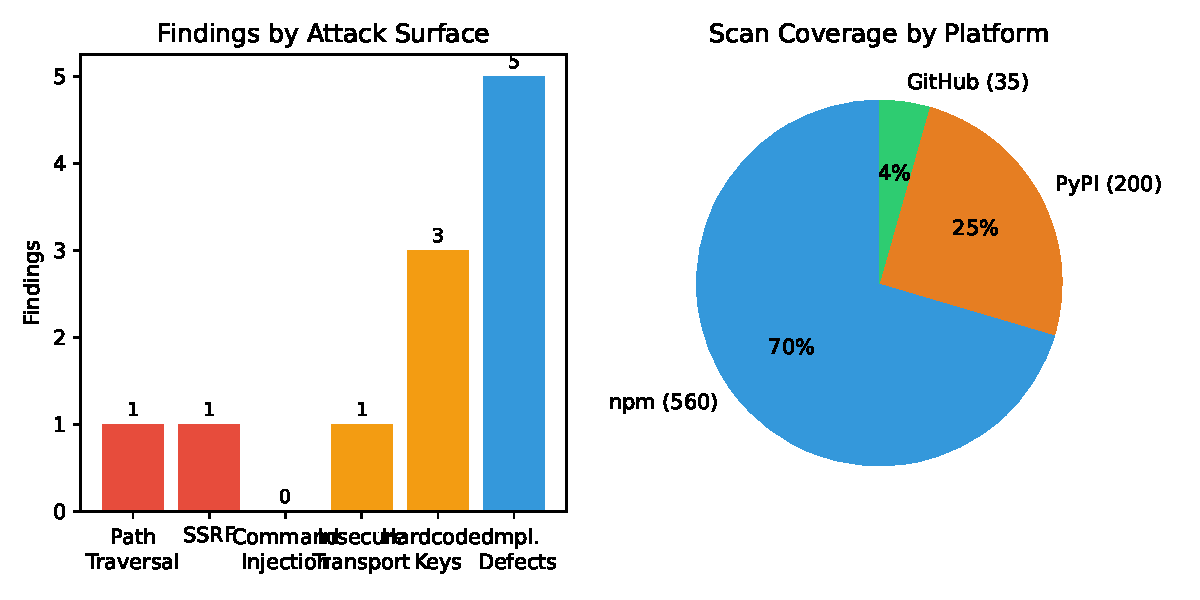
\includegraphics[width=\columnwidth]{../figures/02-mcp-taxonomy/fig1-attack-surfaces.pdf}
\caption{Left: Findings by attack surface. Right: Scan coverage by platform.}
\end{figure}

\section{Results}

\begin{table}[h]
\centering
\caption{Scan Statistics}
\begin{tabular}{l r}
\toprule
Platform & Packages Scanned \\
\midrule
npm (MCP-related) & 560+ \\
PyPI (MCP-related) & 200+ \\
GitHub (topic:mcp-server) & 35+ \\
\midrule
Total & $\sim$800 \\
\bottomrule
\end{tabular}
\end{table}

\section{The 6 Attack Surfaces}

\begin{enumerate}
\item \textbf{AS1: Tool Parameter Injection} — Path traversal, SSRF in tool parameters
\item \textbf{AS2: Inspector Exposure} — Debugging tools bind to 0.0.0.0 without auth
\item \textbf{AS3: Client Trust Exploitation} — Malicious tool descriptions
\item \textbf{AS4: Transport Security} — Plain HTTP, missing TLS
\item \textbf{AS5: Implementation Flaws} — Hardcoded secrets, eval() without sandbox
\item \textbf{AS6: Supply Chain} — No security policy, unpinned dependencies
\end{enumerate}

\section{Conclusion}
The MCP ecosystem has a remarkably low vulnerability rate (0.25\%) but severe impact when vulnerabilities occur. We recommend MCP developers implement input validation at the tool boundary.

\end{document}
